\documentclass{standalone}
\usepackage{tikz}

\begin{document}
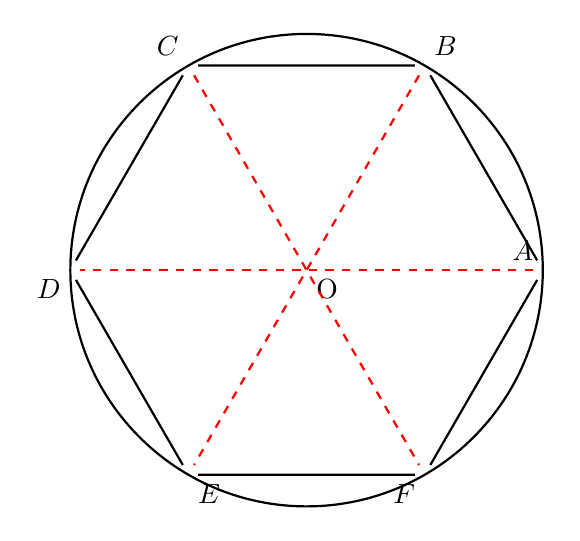
\begin{tikzpicture}[scale=1.5]

% Draw the sphere (circle)
\draw[thick] (0,0) circle (2cm);

% Mark the center point
\node at (0,0) [below right] {O};

% Draw the vertices of the five-point star
\node (A) at (2,0) {};
\node (B) at (1,1.732) {};
\node (C) at (-1,1.732) {};
\node (D) at (-2,0) {};
\node (E) at (-1,-1.732) {};
\node (F) at (1,-1.732) {};

% Draw the edges of the five-point star
\draw[thick] (A) -- (B);
\draw[thick] (B) -- (C);
\draw[thick] (C) -- (D);
\draw[thick] (D) -- (E);
\draw[thick] (E) -- (F);
\draw[thick] (F) -- (A);

% Draw the interlacement graph (bipartite)
\draw[dashed, thick, red] (A) -- (D);
\draw[dashed, thick, red] (B) -- (E);
\draw[dashed, thick, red] (C) -- (F);

% Label the vertices of the interlacement graph
\node at (2,0) [above left] {$A$};
\node at (1,1.732) [above right] {$B$};
\node at (-1,1.732) [above left] {$C$};
\node at (-2,0) [below left] {$D$};
\node at (-1,-1.732) [below right] {$E$};
\node at (1,-1.732) [below left] {$F$};

\end{tikzpicture}
\end{document}